\scanpage{4}

\deleted{\uline{Corollaire} \deleted{\unsure{4.1.1 quater|4.1.2 quater}} Soient $A$ un anneau à spectre irréductible, $\uline{p}$ son unique idéal premier minimal, $B$ une $A$-algèbre de présentation finie $M$ un $B$-module de présentation finie. Supposons que $M_{\uline{p}}$ soit plat,\inserted{sur $A_{\uline{p}}$} alors il existe $f\inserted{\in}A-\uline{p}$ tel que $M_{\uline{f}}$ soit \uline{libre} sur $A_{\uline{f}}$.}

\deleted{\deleted{Supposons d'abord $A$ noethérien, donc $A_{\uline{p}}$ local \uline{artinien}; alors l'hypothèse que $M_{\uline{p}}$ est plat sur $A_{\uline{p}}$} En vertu de \deleted{\unsure{4.1.1 bis}}\inserted{Prop.A}, quitte à remplacer $A$ par un $A_{\uline{f}}$ \deleted{\unsure{aux}} avec $f\quad A-\uline{p}$ convenable, on peut supposer qu'\unsure{il} existe un idéal $J$ \inserted{de type fini} dans $A$ tel que, pour toute $A$-algèbre $A'$, on ait $M\otimes_A A'$ est libre sur $A'$, ou encore plat sur $A'$, sss $A\quad A'$ s'annule sur $J$. Appliquant ceci au cas $A'=A_{\uline{p}}$, on voit que l'on a $JA_{\uline{p}}=0$ i.e. $J_{\uline{p}}=0$. Comme $J$ est de type fini, il s'ensuit qu'il existe $f\quad A-\uline{p}$ tel que $J_{\uline{f}}=0$ i.e. $JA_{\uline{f}}=0$, ce qui implique que $M_{\uline{f}}$ est libre sur $A_{\uline{f}}$, cqfd}

\deleted{Je m'aperçois à l'instant d'une amélioration dans une autre direction de 4.1., dont je vais reprendre l'énoncé:}

\deleted{\uline{Proposition} 4.1. Soient $A$ un anneau, $I$ un idéal \deleted{nilpotent} de $A$, $(A_i)_{i\ I}$ une famille de $A$-algèbres telle que l'intersection des noyaux des homomorphismes $A\quad A_i$ soit réduite à $0$, $M$ un $A$-module. On suppose $M\otimes_A A/I$ libre sur $A/I$ (resp. plat sur $A/I$, \uline{et} l'ensemble d'indices $i$ fini), et pour tout $i$, $M\otimes_A A_i$ libre (resp. plat) sur $A_i$. Alors \inserted{$\forall n$} \inserted{$M\otimes_A(A/I^{\unsure{n+1}})$} $M$ est \deleted{plat sur $A$} libre (resp. plat) sur $A\inserted{/I^{\unsure{n+1}}}$.}

\deleted{Dans le cas non respé, il suffit de prouver aussi la platitude de $M\inserted{_n}$ sur $A\inserted{_n}$, qui entraine la liberté, grâce à \inserted{$M_0=$} $M\otimes_A A/I$ libre et $I$ nilpotent.}

\uline{Corollaire} \deleted{Supposons $A$ \unsure{anneau} \uline{noethérien}\inserted{\deleted{\unsure{noeth.}}}, $M$ un $A$-\unsure{module},}
\deleted{$\unsure{(I_i)_{i\in I}}$ des idéaux de $A$, \inserted{$(\bigcap\unsure{I_i}=0)$} \unsure{$I=\bigcap I_i$} \unsure{tels que} $\forall i$, $M\otimes_A\unsure{A/I_i}$ soit plat sur $\unsure{A_i}$, Alors pour tout entier $n$,}
\unsure{Supposons} \deleted{\unsure{que}} \unsure{qu'on} est dans l'un des cas suivants
\[
\begin{array}{ll}
\text{(i)}&I\text{ nilpotent}\\
\text{(ii)}&A\text{ noeth et }M\text{ idéalement séparé pour }I
\end{array}
\]
Alors \deleted{\unsure{pour les conditions, alors}} $M\text{ plat}/A\Longleftrightarrow\begin{array}{l}\unsure{M_0\text{ libre sur }A_0}\\M_i\text{ plat sur }A_i,\ \forall i.\end{array}$

\margin{\figure{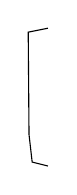
\begin{tikzpicture}\draw (0,0)--(-.2,.05)--(-.24,.4)--(-.25,1.7)--(0,1.75);\end{tikzpicture}}}
\mspage{3}
